%!TEX root = ../MasterThesis.tex

\section{Problem Definition}
\label{sec:problem_definition}

This Master thesis will look into a concept to optimize the collaboration between the affected stakeholders in a case of an existing credit card fraud in an \gls{E-commerce} system. It will \textbf{\underline{not}} look into novel techniques and methods to \textit{prevent} credit card fraud in the \gls{E-commerce} world. This aspect has been seeing a lot of research in the last years.\footnote{Please also note the various US patent applications of Google on that matter from 2015, e.g.:\ “Credit card fraud prevention system and method”, “Financial card fraud alert”, “Payment card fraud prevention system and method” \citep{GooglePatents2015}.}. \\

Stakeholders might include vendors and other businesses, that the retailer has a long-term business relationship with, law enforcement agencies, payment service providers such as PayPal or Visa, banks, and even competitors, that are also affected by the Internet frauds. In such a case the merchant usually tries to solve the issue on their own, and getting in contact with relevant parties by phone or e-mail if necessary. But these communication styles do not fit to the complexity of the task involved, and based on the media-richness model (see Figure~\ref{fig:images_media_richness_model}) will result in inefficient and ineffective problem solutions. \\

\begin{figure}[!ht]
	\centering
		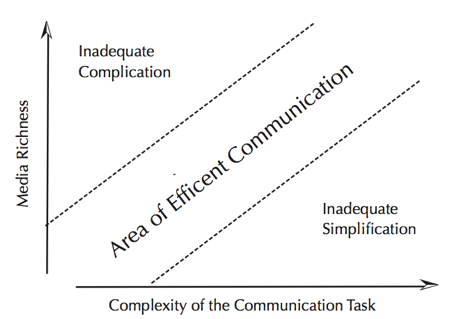
\includegraphics[height=2in]{images/media-richness-model.png}
	\caption{The Media Richness Model \citep{Rice1992}}
\label{fig:images_media_richness_model}
\end{figure}

Due to the task complexity a physical face-to-face meeting with representatives of all stakeholders involved might be a good fit, but arranging such a meeting (same time, same place) with multiple parties, that are globally dispersed, is either economically not feasible or takes a lot of time. But the more time passes for investigating the fraud, the more difficult it will become to identify the fraudsters and take legal actions against them. Acting immediately can therefore reduce the risk of losing the money completely. \\

As of these conditions a computer-supported collaborative work (\gls{CSCW}) system might be an alternative to \textit{cooperate} on an incident of \gls{E-commerce} fraud (same time, different place). \gls{CSCW} systems can be categorized by their support for the mode of group interaction as done in the ``3C model'': \@

\begin{itemize}
    \item\textbf{communication:} two-way exchange of information between different parties
    \item\textbf{coordination:} management of shared resources such as meeting rooms
    \item\textbf{collaboration:} members of a group work together in a shared environment to reach a goal
\end{itemize}

Based on the level of support for one of these functionalities the various systems can be classified and described (see Figure~\ref{fig:images_3C_model}) \citep{Koch2008}: \@

\begin{figure}[H]
	\centering
		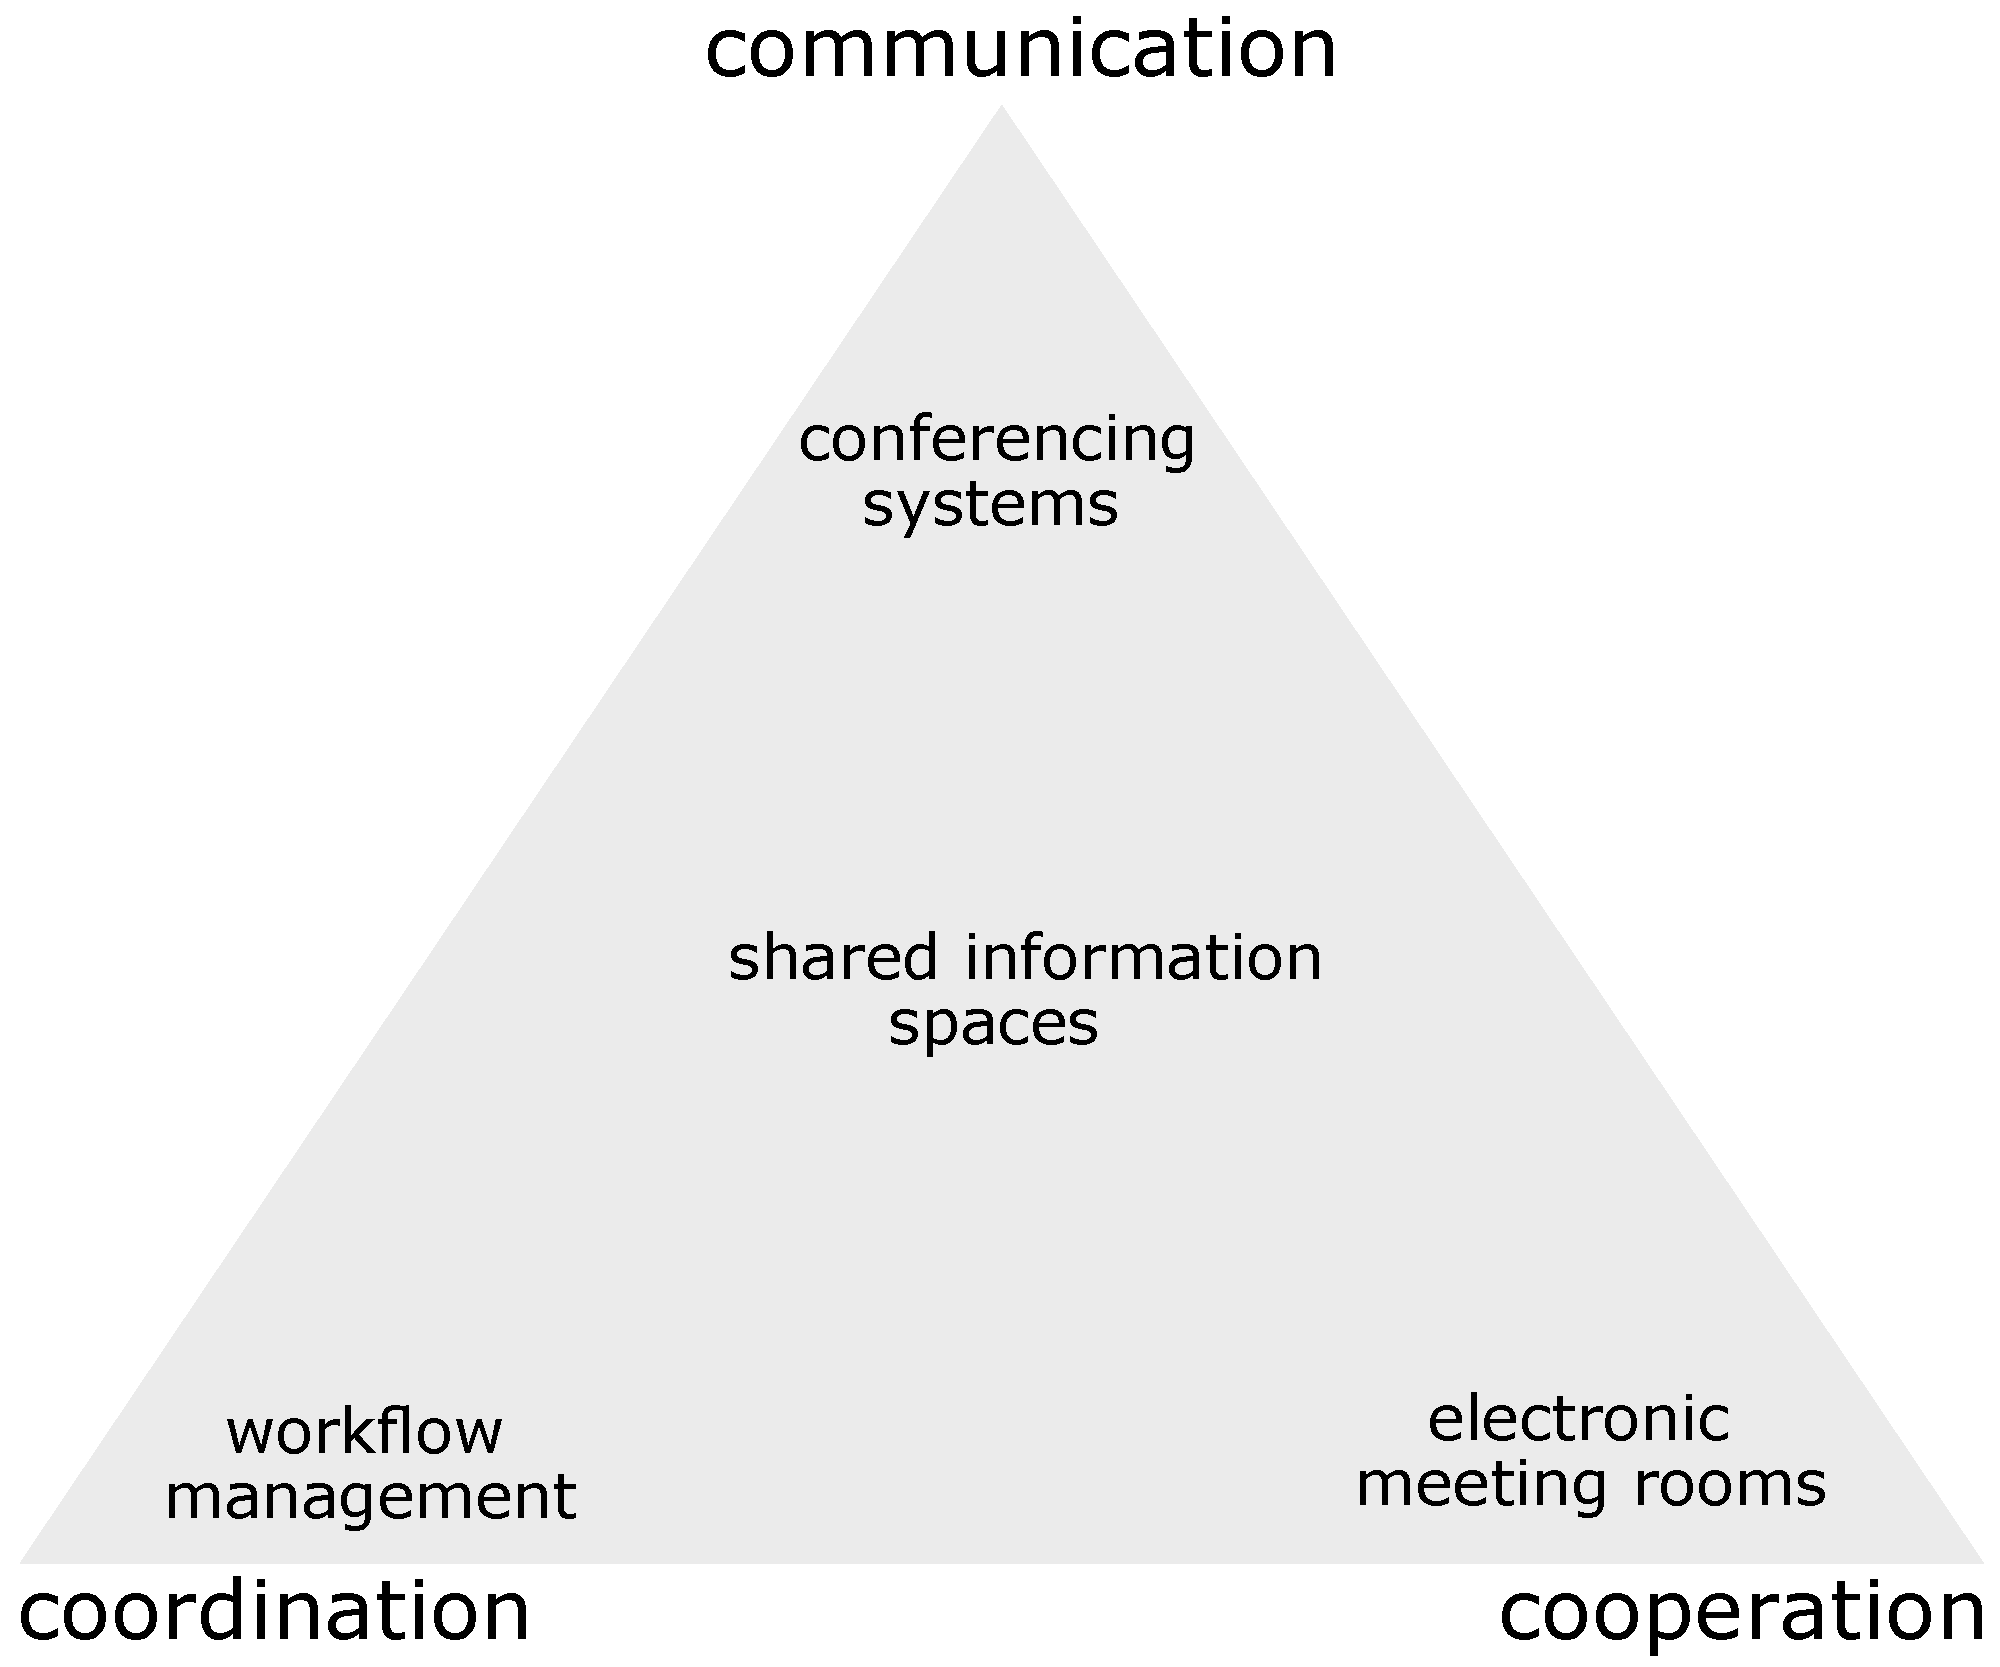
\includegraphics[height=2.5in]{images/3C-model.pdf}
	\caption{The 3C Model \citep{Koch2008}}
\label{fig:images_3C_model}
\end{figure}

A good candidate for such a collaborative system \textbf{\underline{could}} be a shared information space; aka team rooms, cloud storage services or document management systems, that allow participating parties to access information at any place, any time and to share information between each other --- usually with a build in versioning support for artefacts and a workflow component. \\

However, as some of the required information might be confidential or business-critical to one of the involved parties, a centralized system (e.g.\ a service in the cloud) can \textbf{\underline{not}} be used in the scenario described here. Another key characteristic of the investigation of an \gls{E-commerce} fraud is the fact, that it involves information sharing from many different organizations. These different aspects have to be combined into a shared information space in a meaningful way to be able to achieve a common group goal on time. Trying to combine information from different stakeholders will face issues due to different wordings and data formats, competing incentives of the stakeholders to participate on information sharing as well as possible sharing restrictions, that prevent making the information available to a larger audience. \\

Decentralized information sharing architectures, that utilizes peer-to-peer communication technologies, are either restricted to a commonly agreed set of data entities and relations (based on an ontology) between all parties involved, or are lacking richer semantics for sharing and integrating content between the stakeholders. Semantic Web technologies can help lower the barrier to integrate information from various sources into a shared information space, and the advantages of peer-to-peer communication and Semantic Web technologies for information sharing in distributed, inter-organizational settings have been shown in \citep{Staab2006}. \\

Still these studies concentrate on making information from different parties searchable and accessible in a distributed, shared information space, in which data can be accessed and queried at any time from any participating party. They are not solving the problem of working collaboratively on a common goal in an ad-hoc, loosely-coupled virtual team of disperse organizations by making certain (sometimes sensitive) information available in a shared environment. \\

Therefore, the research question for this Master thesis can be summarized as follows: \\[3em]

\begin{quotation}
  \textit{In how far can a computer supported collaborative work system based on peer-to-peer communication and Semantic Web technologies improve the efficiency and effectivity of \gls{E-commerce} fraud investigations within an inter-institutional team?}
\end{quotation}

% section problem definition (end)
